\documentclass{standalone}
\usepackage{tikz}
\usetikzlibrary{patterns, positioning}
\usepackage[sfdefault]{ClearSans} %% option 'sfdefault' activates Clear Sans as the default text font
\usepackage[T1]{fontenc}

\begin{document}
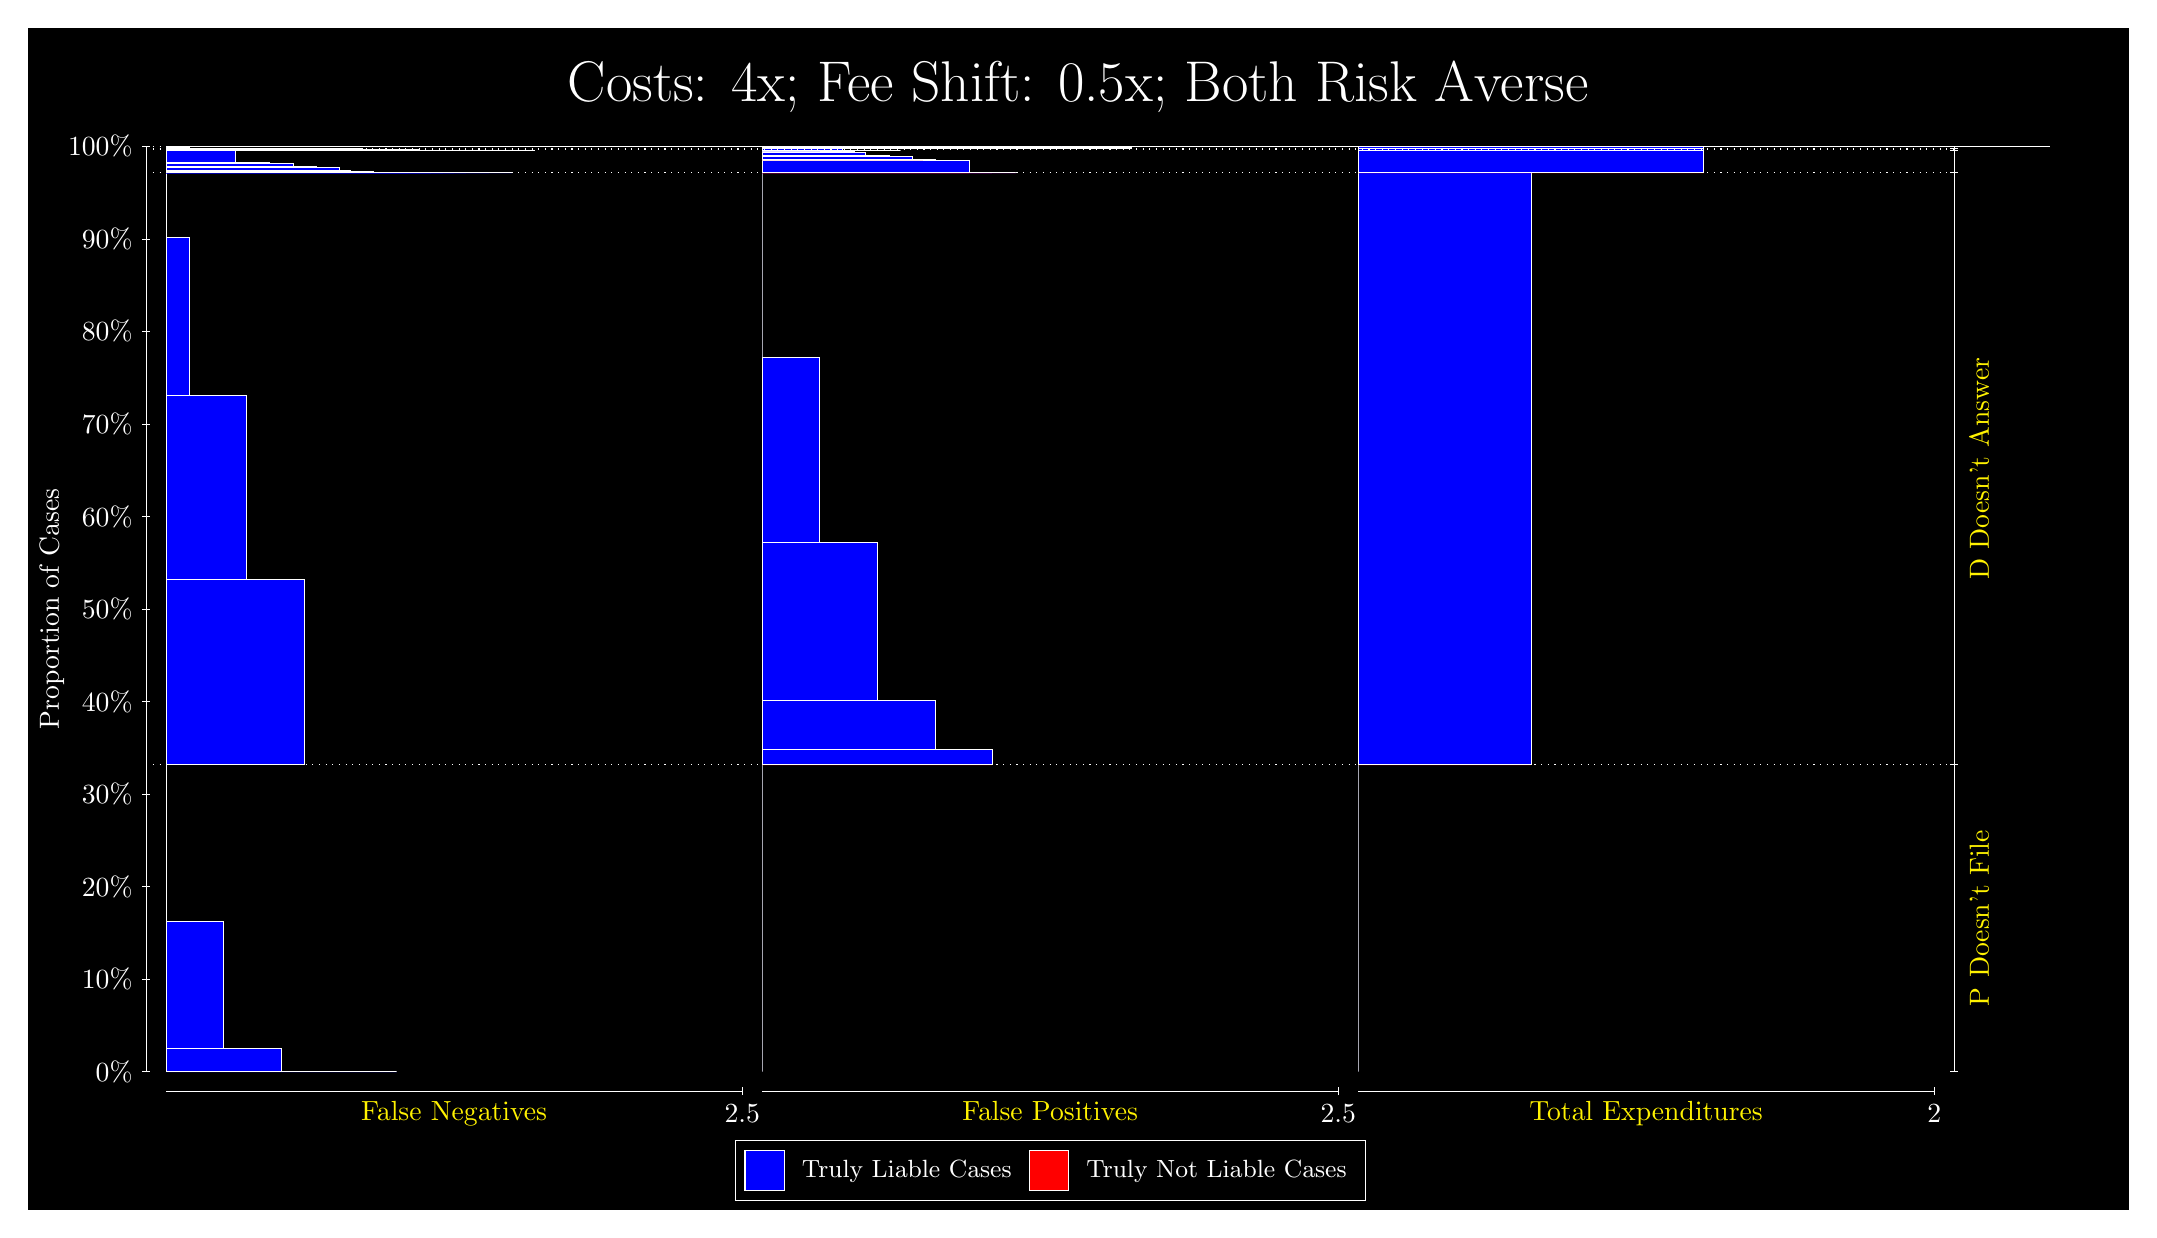
\begin{tikzpicture}
\draw[fill=black] (0,0) rectangle (26.667,15);
\draw[text=white] (0,13.5) rectangle (26.667,15) node[midway] {\huge Costs: 4x; Fee Shift: 0.5x; Both Risk Averse};
\draw[white, very thin] (1.5,1.75) -- (1.5,13.5);
\node[rotate=90, text=white, anchor=center] at (0.3, 7.625) {Proportion of Cases};
\draw[white, very thin] (1.45,1.75) -- (1.55,1.75);
\node[text=white, anchor=east] at (1.45, 1.75) {0\%};
\draw[white, very thin] (1.45,2.925) -- (1.55,2.925);
\node[text=white, anchor=east] at (1.45, 2.925) {10\%};
\draw[white, very thin] (1.45,4.1) -- (1.55,4.1);
\node[text=white, anchor=east] at (1.45, 4.1) {20\%};
\draw[white, very thin] (1.45,5.275) -- (1.55,5.275);
\node[text=white, anchor=east] at (1.45, 5.275) {30\%};
\draw[white, very thin] (1.45,6.45) -- (1.55,6.45);
\node[text=white, anchor=east] at (1.45, 6.45) {40\%};
\draw[white, very thin] (1.45,7.625) -- (1.55,7.625);
\node[text=white, anchor=east] at (1.45, 7.625) {50\%};
\draw[white, very thin] (1.45,8.8) -- (1.55,8.8);
\node[text=white, anchor=east] at (1.45, 8.8) {60\%};
\draw[white, very thin] (1.45,9.975) -- (1.55,9.975);
\node[text=white, anchor=east] at (1.45, 9.975) {70\%};
\draw[white, very thin] (1.45,11.15) -- (1.55,11.15);
\node[text=white, anchor=east] at (1.45, 11.15) {80\%};
\draw[white, very thin] (1.45,12.325) -- (1.55,12.325);
\node[text=white, anchor=east] at (1.45, 12.325) {90\%};
\draw[white, very thin] (1.45,13.5) -- (1.55,13.5);
\node[text=white, anchor=east] at (1.45, 13.5) {100\%};

\draw[white, very thin] (24.457,1.75) -- (24.457,13.5);
\draw[white, very thin] (24.407,1.75) -- (24.507,1.75);
\node[anchor=west] at (24.407, 1.75) {};
\draw[white, very thin] (24.407,5.6469) -- (24.507,5.6469);
\node[anchor=west] at (24.407, 5.6469) {};
\draw[white, very thin] (24.407,13.165) -- (24.507,13.165);
\node[anchor=west] at (24.407, 13.165) {};
\draw[white, very thin] (24.407,13.456) -- (24.507,13.456);
\node[anchor=west] at (24.407, 13.456) {};
\draw[white, very thin] (24.407,13.478) -- (24.507,13.478);
\node[anchor=west] at (24.407, 13.478) {};
\draw[white, very thin] (24.407,13.498) -- (24.507,13.498);
\node[anchor=west] at (24.407, 13.498) {};
\draw[white, very thin] (24.407,13.5) -- (24.507,13.5);
\node[anchor=west] at (24.407, 13.5) {};

\draw[white, very thin, fill=blue] (1.75,1.75) rectangle (4.6775,1.75);
\draw[white, very thin, fill=blue] (1.75,1.75) rectangle (3.9457,1.7525);
\draw[white, very thin, fill=blue] (1.75,1.7525) rectangle (3.2138,2.051);
\draw[white, very thin, fill=blue] (1.75,2.051) rectangle (2.4819,3.6547);
\draw[white, very thin, fill=red] (1.75,3.6547) rectangle (1.75,3.6547);
\draw[white, very thin, fill=blue] (1.75,3.6547) rectangle (1.75,5.6469);
\draw[white, very thin, fill=blue] (1.75,5.6469) rectangle (3.5065,7.9968);
\draw[white, very thin, fill=blue] (1.75,7.9968) rectangle (2.7746,10.344);
\draw[white, very thin, fill=blue] (1.75,10.344) rectangle (2.0428,12.35);
\draw[white, very thin, fill=red] (1.75,12.35) rectangle (1.75,12.35);
\draw[white, very thin, fill=blue] (1.75,12.35) rectangle (1.75,13.165);
\draw[white, very thin, fill=blue] (1.75,13.165) rectangle (6.1413,13.165);
\draw[white, very thin, fill=blue] (1.75,13.165) rectangle (5.8486,13.165);
\draw[white, very thin, fill=blue] (1.75,13.165) rectangle (5.5558,13.165);
\draw[white, very thin, fill=blue] (1.75,13.165) rectangle (5.4094,13.165);
\draw[white, very thin, fill=blue] (1.75,13.165) rectangle (5.2631,13.165);
\draw[white, very thin, fill=blue] (1.75,13.165) rectangle (5.1167,13.165);
\draw[white, very thin, fill=blue] (1.75,13.165) rectangle (4.9703,13.165);
\draw[white, very thin, fill=blue] (1.75,13.165) rectangle (4.8239,13.165);
\draw[white, very thin, fill=blue] (1.75,13.165) rectangle (4.6775,13.175);
\draw[white, very thin, fill=blue] (1.75,13.175) rectangle (4.5312,13.175);
\draw[white, very thin, fill=blue] (1.75,13.175) rectangle (4.3848,13.183);
\draw[white, very thin, fill=blue] (1.75,13.183) rectangle (4.2384,13.183);
\draw[white, very thin, fill=blue] (1.75,13.183) rectangle (4.092,13.191);
\draw[white, very thin, fill=blue] (1.75,13.191) rectangle (3.9457,13.232);
\draw[white, very thin, fill=blue] (1.75,13.232) rectangle (3.7993,13.238);
\draw[white, very thin, fill=blue] (1.75,13.238) rectangle (3.6529,13.246);
\draw[white, very thin, fill=blue] (1.75,13.246) rectangle (3.5065,13.249);
\draw[white, very thin, fill=blue] (1.75,13.249) rectangle (3.3602,13.288);
\draw[white, very thin, fill=blue] (1.75,13.288) rectangle (3.2138,13.289);
\draw[white, very thin, fill=blue] (1.75,13.289) rectangle (3.0674,13.295);
\draw[white, very thin, fill=blue] (1.75,13.295) rectangle (2.921,13.295);
\draw[white, very thin, fill=blue] (1.75,13.295) rectangle (2.7746,13.296);
\draw[white, very thin, fill=blue] (1.75,13.296) rectangle (2.6283,13.456);
\draw[white, very thin, fill=blue] (1.75,13.456) rectangle (2.3355,13.456);
\draw[white, very thin, fill=blue] (1.75,13.456) rectangle (2.0428,13.456);
\draw[white, very thin, fill=red] (1.75,13.456) rectangle (1.75,13.456);
\draw[white, very thin, fill=blue] (1.75,13.456) rectangle (6.4341,13.456);
\draw[white, very thin, fill=blue] (1.75,13.456) rectangle (5.7022,13.456);
\draw[white, very thin, fill=blue] (1.75,13.456) rectangle (4.9703,13.46);
\draw[white, very thin, fill=blue] (1.75,13.46) rectangle (4.2384,13.477);
\draw[white, very thin, fill=blue] (1.75,13.477) rectangle (3.5065,13.478);
\draw[white, very thin, fill=red] (1.75,13.478) rectangle (1.75,13.478);
\draw[white, very thin, fill=blue] (1.75,13.478) rectangle (3.5065,13.478);
\draw[white, very thin, fill=blue] (1.75,13.478) rectangle (2.7746,13.478);
\draw[white, very thin, fill=blue] (1.75,13.478) rectangle (2.0428,13.484);
\draw[white, very thin, fill=red] (1.75,13.484) rectangle (1.75,13.484);
\draw[white, very thin, fill=blue] (1.75,13.484) rectangle (1.75,13.498);
\draw[white, very thin, fill=blue] (1.75,13.498) rectangle (9.9471,13.498);
\draw[white, very thin, fill=blue] (1.75,13.498) rectangle (9.2152,13.498);
\draw[white, very thin, fill=blue] (1.75,13.498) rectangle (8.4834,13.498);
\draw[white, very thin, fill=blue] (1.75,13.498) rectangle (7.7515,13.499);
\draw[white, very thin, fill=blue] (1.75,13.499) rectangle (7.0196,13.499);
\draw[white, very thin, fill=blue] (1.75,13.499) rectangle (6.2877,13.499);
\draw[white, very thin, fill=blue] (1.75,13.499) rectangle (5.7022,13.499);
\draw[white, very thin, fill=blue] (1.75,13.499) rectangle (4.9703,13.499);
\draw[white, very thin, fill=blue] (1.75,13.499) rectangle (4.2384,13.499);
\draw[white, very thin, fill=blue] (1.75,13.499) rectangle (3.5065,13.5);
\draw[white, very thin, fill=blue] (1.75,13.5) rectangle (2.7746,13.5);
\draw[white, very thin, fill=blue] (1.75,13.5) rectangle (2.0428,13.5);
\draw[white, very thin, fill=red] (1.75,13.5) rectangle (1.75,13.5);
\draw[white, very thin, fill=blue] (1.75,13.5) rectangle (1.75,13.5);
\draw[white, very thin, fill=red] (9.3189,1.75) rectangle (9.3189,1.75);
\draw[white, very thin, fill=blue] (9.3189,1.75) rectangle (9.3189,5.6469);
\draw[white, very thin, fill=red] (9.3189,5.6469) rectangle (12.246,5.6469);
\draw[white, very thin, fill=blue] (9.3189,5.6469) rectangle (12.246,5.8382);
\draw[white, very thin, fill=blue] (9.3189,5.8382) rectangle (11.515,6.462);
\draw[white, very thin, fill=blue] (9.3189,6.462) rectangle (10.783,8.4681);
\draw[white, very thin, fill=blue] (9.3189,8.4681) rectangle (10.051,10.815);
\draw[white, very thin, fill=blue] (9.3189,10.815) rectangle (9.3189,13.165);
\draw[white, very thin, fill=red] (9.3189,13.165) rectangle (12.539,13.165);
\draw[white, very thin, fill=blue] (9.3189,13.165) rectangle (12.539,13.165);
\draw[white, very thin, fill=red] (9.3189,13.165) rectangle (12.246,13.165);
\draw[white, very thin, fill=blue] (9.3189,13.165) rectangle (12.246,13.165);
\draw[white, very thin, fill=red] (9.3189,13.165) rectangle (11.954,13.165);
\draw[white, very thin, fill=blue] (9.3189,13.165) rectangle (11.954,13.324);
\draw[white, very thin, fill=blue] (9.3189,13.324) rectangle (11.807,13.325);
\draw[white, very thin, fill=red] (9.3189,13.325) rectangle (11.661,13.325);
\draw[white, very thin, fill=blue] (9.3189,13.325) rectangle (11.661,13.325);
\draw[white, very thin, fill=blue] (9.3189,13.325) rectangle (11.515,13.331);
\draw[white, very thin, fill=red] (9.3189,13.331) rectangle (11.368,13.331);
\draw[white, very thin, fill=blue] (9.3189,13.331) rectangle (11.368,13.333);
\draw[white, very thin, fill=blue] (9.3189,13.333) rectangle (11.222,13.372);
\draw[white, very thin, fill=blue] (9.3189,13.372) rectangle (11.075,13.374);
\draw[white, very thin, fill=blue] (9.3189,13.374) rectangle (10.929,13.382);
\draw[white, very thin, fill=blue] (9.3189,13.382) rectangle (10.783,13.389);
\draw[white, very thin, fill=blue] (9.3189,13.389) rectangle (10.636,13.429);
\draw[white, very thin, fill=blue] (9.3189,13.429) rectangle (10.49,13.438);
\draw[white, very thin, fill=blue] (9.3189,13.438) rectangle (10.344,13.438);
\draw[white, very thin, fill=blue] (9.3189,13.438) rectangle (10.197,13.446);
\draw[white, very thin, fill=blue] (9.3189,13.446) rectangle (10.051,13.446);
\draw[white, very thin, fill=blue] (9.3189,13.446) rectangle (9.9044,13.456);
\draw[white, very thin, fill=blue] (9.3189,13.456) rectangle (9.758,13.456);
\draw[white, very thin, fill=blue] (9.3189,13.456) rectangle (9.6116,13.456);
\draw[white, very thin, fill=blue] (9.3189,13.456) rectangle (9.4652,13.456);
\draw[white, very thin, fill=blue] (9.3189,13.456) rectangle (9.3189,13.456);
\draw[white, very thin, fill=red] (9.3189,13.456) rectangle (11.075,13.456);
\draw[white, very thin, fill=blue] (9.3189,13.456) rectangle (11.075,13.456);
\draw[white, very thin, fill=blue] (9.3189,13.456) rectangle (10.344,13.474);
\draw[white, very thin, fill=blue] (9.3189,13.474) rectangle (9.6116,13.478);
\draw[white, very thin, fill=blue] (9.3189,13.478) rectangle (9.3189,13.478);
\draw[white, very thin, fill=red] (9.3189,13.478) rectangle (14.003,13.478);
\draw[white, very thin, fill=blue] (9.3189,13.478) rectangle (14.003,13.482);
\draw[white, very thin, fill=blue] (9.3189,13.482) rectangle (13.271,13.492);
\draw[white, very thin, fill=blue] (9.3189,13.492) rectangle (12.539,13.498);
\draw[white, very thin, fill=blue] (9.3189,13.498) rectangle (11.807,13.498);
\draw[white, very thin, fill=blue] (9.3189,13.498) rectangle (11.075,13.498);
\draw[white, very thin, fill=red] (9.3189,13.498) rectangle (17.516,13.498);
\draw[white, very thin, fill=blue] (9.3189,13.498) rectangle (17.516,13.498);
\draw[white, very thin, fill=red] (9.3189,13.498) rectangle (16.784,13.498);
\draw[white, very thin, fill=blue] (9.3189,13.498) rectangle (16.784,13.498);
\draw[white, very thin, fill=red] (9.3189,13.498) rectangle (16.052,13.498);
\draw[white, very thin, fill=blue] (9.3189,13.498) rectangle (16.052,13.498);
\draw[white, very thin, fill=red] (9.3189,13.498) rectangle (15.32,13.498);
\draw[white, very thin, fill=blue] (9.3189,13.498) rectangle (15.32,13.499);
\draw[white, very thin, fill=blue] (9.3189,13.499) rectangle (14.588,13.499);
\draw[white, very thin, fill=blue] (9.3189,13.499) rectangle (13.857,13.499);
\draw[white, very thin, fill=blue] (9.3189,13.499) rectangle (13.125,13.499);
\draw[white, very thin, fill=blue] (9.3189,13.499) rectangle (12.393,13.499);
\draw[white, very thin, fill=red] (9.3189,13.499) rectangle (11.807,13.499);
\draw[white, very thin, fill=blue] (9.3189,13.499) rectangle (11.807,13.499);
\draw[white, very thin, fill=red] (9.3189,13.499) rectangle (11.075,13.499);
\draw[white, very thin, fill=blue] (9.3189,13.499) rectangle (11.075,13.5);
\draw[white, very thin, fill=blue] (9.3189,13.5) rectangle (10.344,13.5);
\draw[white, very thin, fill=blue] (9.3189,13.5) rectangle (9.6116,13.5);
\draw[white, very thin, fill=blue] (9.3189,13.5) rectangle (9.3189,13.5);
\draw[white, very thin, fill=red] (16.888,1.75) rectangle (16.888,1.75);
\draw[white, very thin, fill=blue] (16.888,1.75) rectangle (16.888,5.6469);
\draw[white, very thin, fill=red] (16.888,5.6469) rectangle (19.083,5.6469);
\draw[white, very thin, fill=blue] (16.888,5.6469) rectangle (19.083,13.165);
\draw[white, very thin, fill=red] (16.888,13.165) rectangle (21.279,13.165);
\draw[white, very thin, fill=blue] (16.888,13.165) rectangle (21.279,13.168);
\draw[white, very thin, fill=red] (16.888,13.168) rectangle (21.279,13.168);
\draw[white, very thin, fill=blue] (16.888,13.168) rectangle (21.279,13.456);
\draw[white, very thin, fill=red] (16.888,13.456) rectangle (21.279,13.456);
\draw[white, very thin, fill=blue] (16.888,13.456) rectangle (21.279,13.478);
\draw[white, very thin, fill=red] (16.888,13.478) rectangle (21.279,13.478);
\draw[white, very thin, fill=blue] (16.888,13.478) rectangle (21.279,13.498);
\draw[white, very thin, fill=red] (16.888,13.498) rectangle (25.67,13.498);
\draw[white, very thin, fill=blue] (16.888,13.498) rectangle (25.67,13.5);
\draw[white, dotted] (1.5,5.6469) -- (24.457,5.6469);
\draw[white, dotted] (1.5,13.165) -- (24.457,13.165);
\draw[white, dotted] (1.5,13.456) -- (24.457,13.456);
\draw[white, dotted] (1.5,13.478) -- (24.457,13.478);
\draw[white, dotted] (1.5,13.498) -- (24.457,13.498);
\draw[white, very thin] (1.75,1.5) -- (9.0689,1.5);
\node[text=yellow, anchor=north] at (5.4094, 1.5) {False Negatives};
\draw[white, very thin] (9.0689,1.45) -- (9.0689,1.55);
\node[text=white, anchor=north] at (9.0689, 1.45) {2.5};

\draw[white, very thin] (9.3189,1.5) -- (16.638,1.5);
\node[text=yellow, anchor=north] at (12.978, 1.5) {False Positives};
\draw[white, very thin] (16.638,1.45) -- (16.638,1.55);
\node[text=white, anchor=north] at (16.638, 1.45) {2.5};

\draw[white, very thin] (16.888,1.5) -- (24.207,1.5);
\node[text=yellow, anchor=north] at (20.547, 1.5) {Total Expenditures};
\draw[white, very thin] (24.207,1.45) -- (24.207,1.55);
\node[text=white, anchor=north] at (24.207, 1.45) {2};

\node[text=yellow, centered, rotate=90] at (24.777, 3.6984) {P Doesn't File};
\node[text=yellow, centered, rotate=90] at (24.777, 9.4059) {D Doesn't Answer};





\draw (12.978300999999998,1.5) node[draw=none] (baseCoordinate) {};
\begin{scope}[align=center]
        \matrix[scale=0.5, draw=white, below=0.5cm of baseCoordinate, nodes={draw}, column sep=0.1cm]{
            \node[rectangle, draw, minimum width=0.5cm, minimum height=0.5cm, fill=blue] {}; &
            \node[draw=none, font=\small, text=white] (B) {Truly Liable Cases}; &
            \node[rectangle, draw, minimum width=0.5cm, minimum height=0.5cm, fill=red] {}; &
            \node[draw=none, font=\small, text=white] (B) {Truly Not Liable Cases}; \\
            };
\end{scope}

\end{tikzpicture}
\end{document}